\addtocontents{toc}{\protect\vspace{\beforebibskip}} % Place slightly below the rest of the document content in the table


%************************************************
\chapter{Desenvolvimento}
\label{ch:desenvolvimento}
%************************************************

O corpo do relatório constitui a parte mais extensa do trabalho e deve conter o desenvolvimento das ideias referidas na Introdução. Nesta parte do relatório incluem-se o assunto, objeto a ser tratado, a metodologia da sequência de exposição, a descrição dos métodos e técnicas usados, a construção de argumentos, a explicação de conceitos e noções, a análise e a interpretação de dados.
 
\section{Estilos}

O \LaTeXe\ trata da formação, apenas temos de usar as \emph{tags} correctas. Seguem-se alguns exemplos. 

A Figura \ref{fig:terrenos} é constituída por 3 imagens em ficheiros \textbf{.jpg} separados. A Figura \ref{fig:vulcao} é constituída apenas por um ficheiro e ocupa 50\% da largura de uma linha de texto.


% Ao omitirmos a extensão do ficheiro de imagem estamos a permitir que 
% seja possível compilar o ficheiro com Latex ou PDFLatex
% em contrapartida temos de ter 2 vezes a mesma imagem:
% 	- .eps para o Latex
% 	- .jpg ou .pdf para o PDFLatex
\begin{figure}
 \centering
 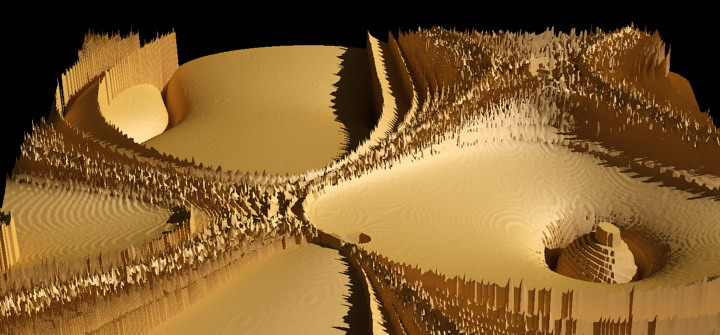
\includegraphics[width=0.32\linewidth]{imgs/tp04a_450}
 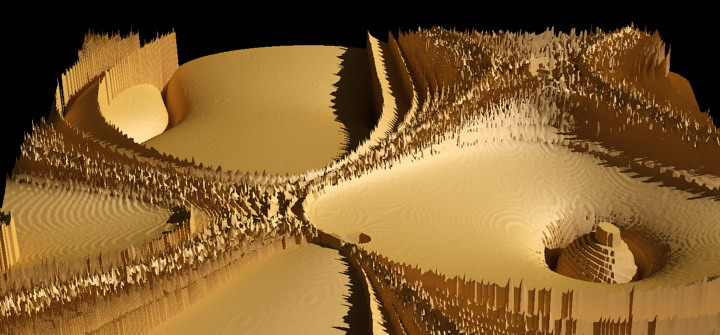
\includegraphics[width=0.32\linewidth]{imgs/tp04a_450}
 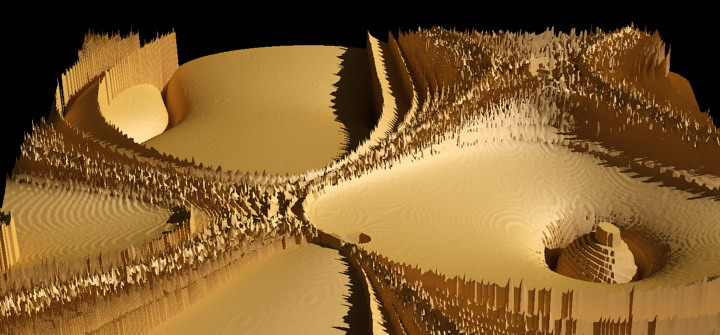
\includegraphics[width=0.32\linewidth]{imgs/tp04a_450}
 % tp04a_450.jpg: 720x335 pixel, 72dpi, 25.40x11.82 cm, bb=0 0 720 335
 \caption[Imagem composta]{Imagem composta por três figuras em ficheiros separados}
 \label{fig:terrenos}
\end{figure}


\begin{figure}
 \centering
 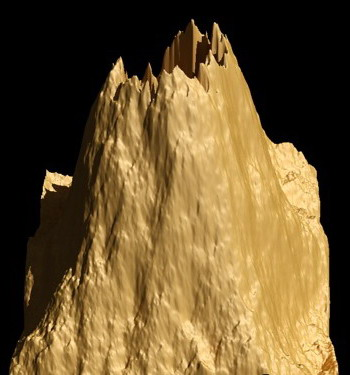
\includegraphics[width=0.5\linewidth]{imgs/tp45a_450}
 % tp45a_450.eps: 1179666x1179666 pixel, 300dpi, 9987.84x9987.84 cm, bb=20 20 575 615
 \caption{Vulcão}
 \label{fig:vulcao}
\end{figure}


Na Tabela \ref{tableBenchmark} apresenta-se um exemplo de uma tabela.

\begin{table}
  \caption[Exemplo de uma tabela]{Floating point benchmark.
	\textbf{R$_{max}$}: the performance in Gflops for the largest problem run on a machine;
	\textbf{N$_{max}$}: the size of the largest problem run on a machine;
	\textbf{N$_{1/2}$}: the size where half the R$_{max}$ execution rate is achieved;
	\textbf{R$_{peak}$}: the theoretical peak performance in Gflops for the machine}
  \label{tableBenchmark}
  \begin{center} 
  \begin{tabular*}{1\textwidth}{@{\extracolsep{\fill}} rccccc } \toprule
\textbf{Linpack	Benchmark}& Proc.	& \textbf{R$_{max}$} & \textbf{N$_{max}$} & \textbf{N$_{1/2}$}	& \textbf{R$_{peak}$} \\ 
(Full precision)	& or Cores	& GFlops	     & Order		  & Order		& GFlops \\ [0.25ex] \midrule
Thinking Machine CM-5	& 32		& 1,900		     & 9216		  & 4096		& 4 \\
Pentium 4 3.0 GHz & 1	& 4,730		     & 7600		  & 365			& 6 \\
\multirow{2}{*}{IBM Cell BE 3.2 GHz} 	& \multirow{2}{*}{9}& \multirow{2}{*}{98,05} & \multirow{2}{*}{4096} & \multirow{2}{*}{1536} & 204,8 {\scriptsize{(32 bits)}} \\
			&		&		     &			  &			& 14,6 {\scriptsize{(64 bits)}} \\ \bottomrule
  \end{tabular*}
  \end{center}	
\end{table}